\documentclass[12pt]{article}
\usepackage[utf8]{inputenc}
\usepackage{amsmath, amssymb, amsthm}
\usepackage{graphicx}
\usepackage{caption}
\usepackage{subcaption}
\usepackage{booktabs}
\usepackage[margin=1in]{geometry}
\usepackage{enumitem}
\usepackage{float}

\usepackage[colorlinks=true]{hyperref} % Improved hyperref setup

% Add this package to help with reference resolution
\usepackage{bookmark}

\title{ECS 111 Homework Assignment \#3}
\author{Kevin Oghalai}
\date{\today}

\begin{document}

\maketitle
\section{Introduction}
A logistic regression model and Multi Layer Peceptron(MLP) were used to predict 
a movie watchers rating of a movie. The dataset contained the user's ID, 
rating, and timestamp, as well as the movie's ID, title, release date, and genres.
The algorithms stated above were able to achieve roughly a 40\% accuracy of guessing the 
rating, resulting in a RMSE value of roughly 1.1. 

\section{Data Processing}
After the data was loaded in and the movie and user data was matched 
together, the data was split into a training and testing set, with 80\% of the data
being used for training and 20\% being used for testing. 
Values which could be normalized were, and genres and other categorical data were
one-hot encoded, with each genre being represented by a binary value. 
Additionally, the data had its dimensionality reduced using Singular 
Value Decomposition (SVD) to reduce the number of features and compare the 
performance of the model with and without SVD. 



\section{Results}
The logistic regression model was fairly consistent, with hyperparameter tuning
not changing the results significantly. The model was able to achieve a 1.045 RMSE 
on the training set, 1.139 RMSE on the validation set, and 1.123 RMSE on the test set. 
Results are shown in Table \ref{tab:results}.

The Multi Layer Perceptron (MLP) model had 3 fully connected layers 
with ReLU activation 
functions in between. There were 500 neurons in each layer, although results
were very similar when testing with both 100 and 1000 neurons.
Cross entropy loss was used with the ADAM optimizer. 
The MLP model was more sensitive to 
hyperparameter tuning, with changes in training time vastly 
decreasing the validation accuracy. A plot of the validation 
accuracy vs. training time is shown in Figure \ref{fig:mlp_val_acc}. 

\begin{figure}[H]
    \centering
    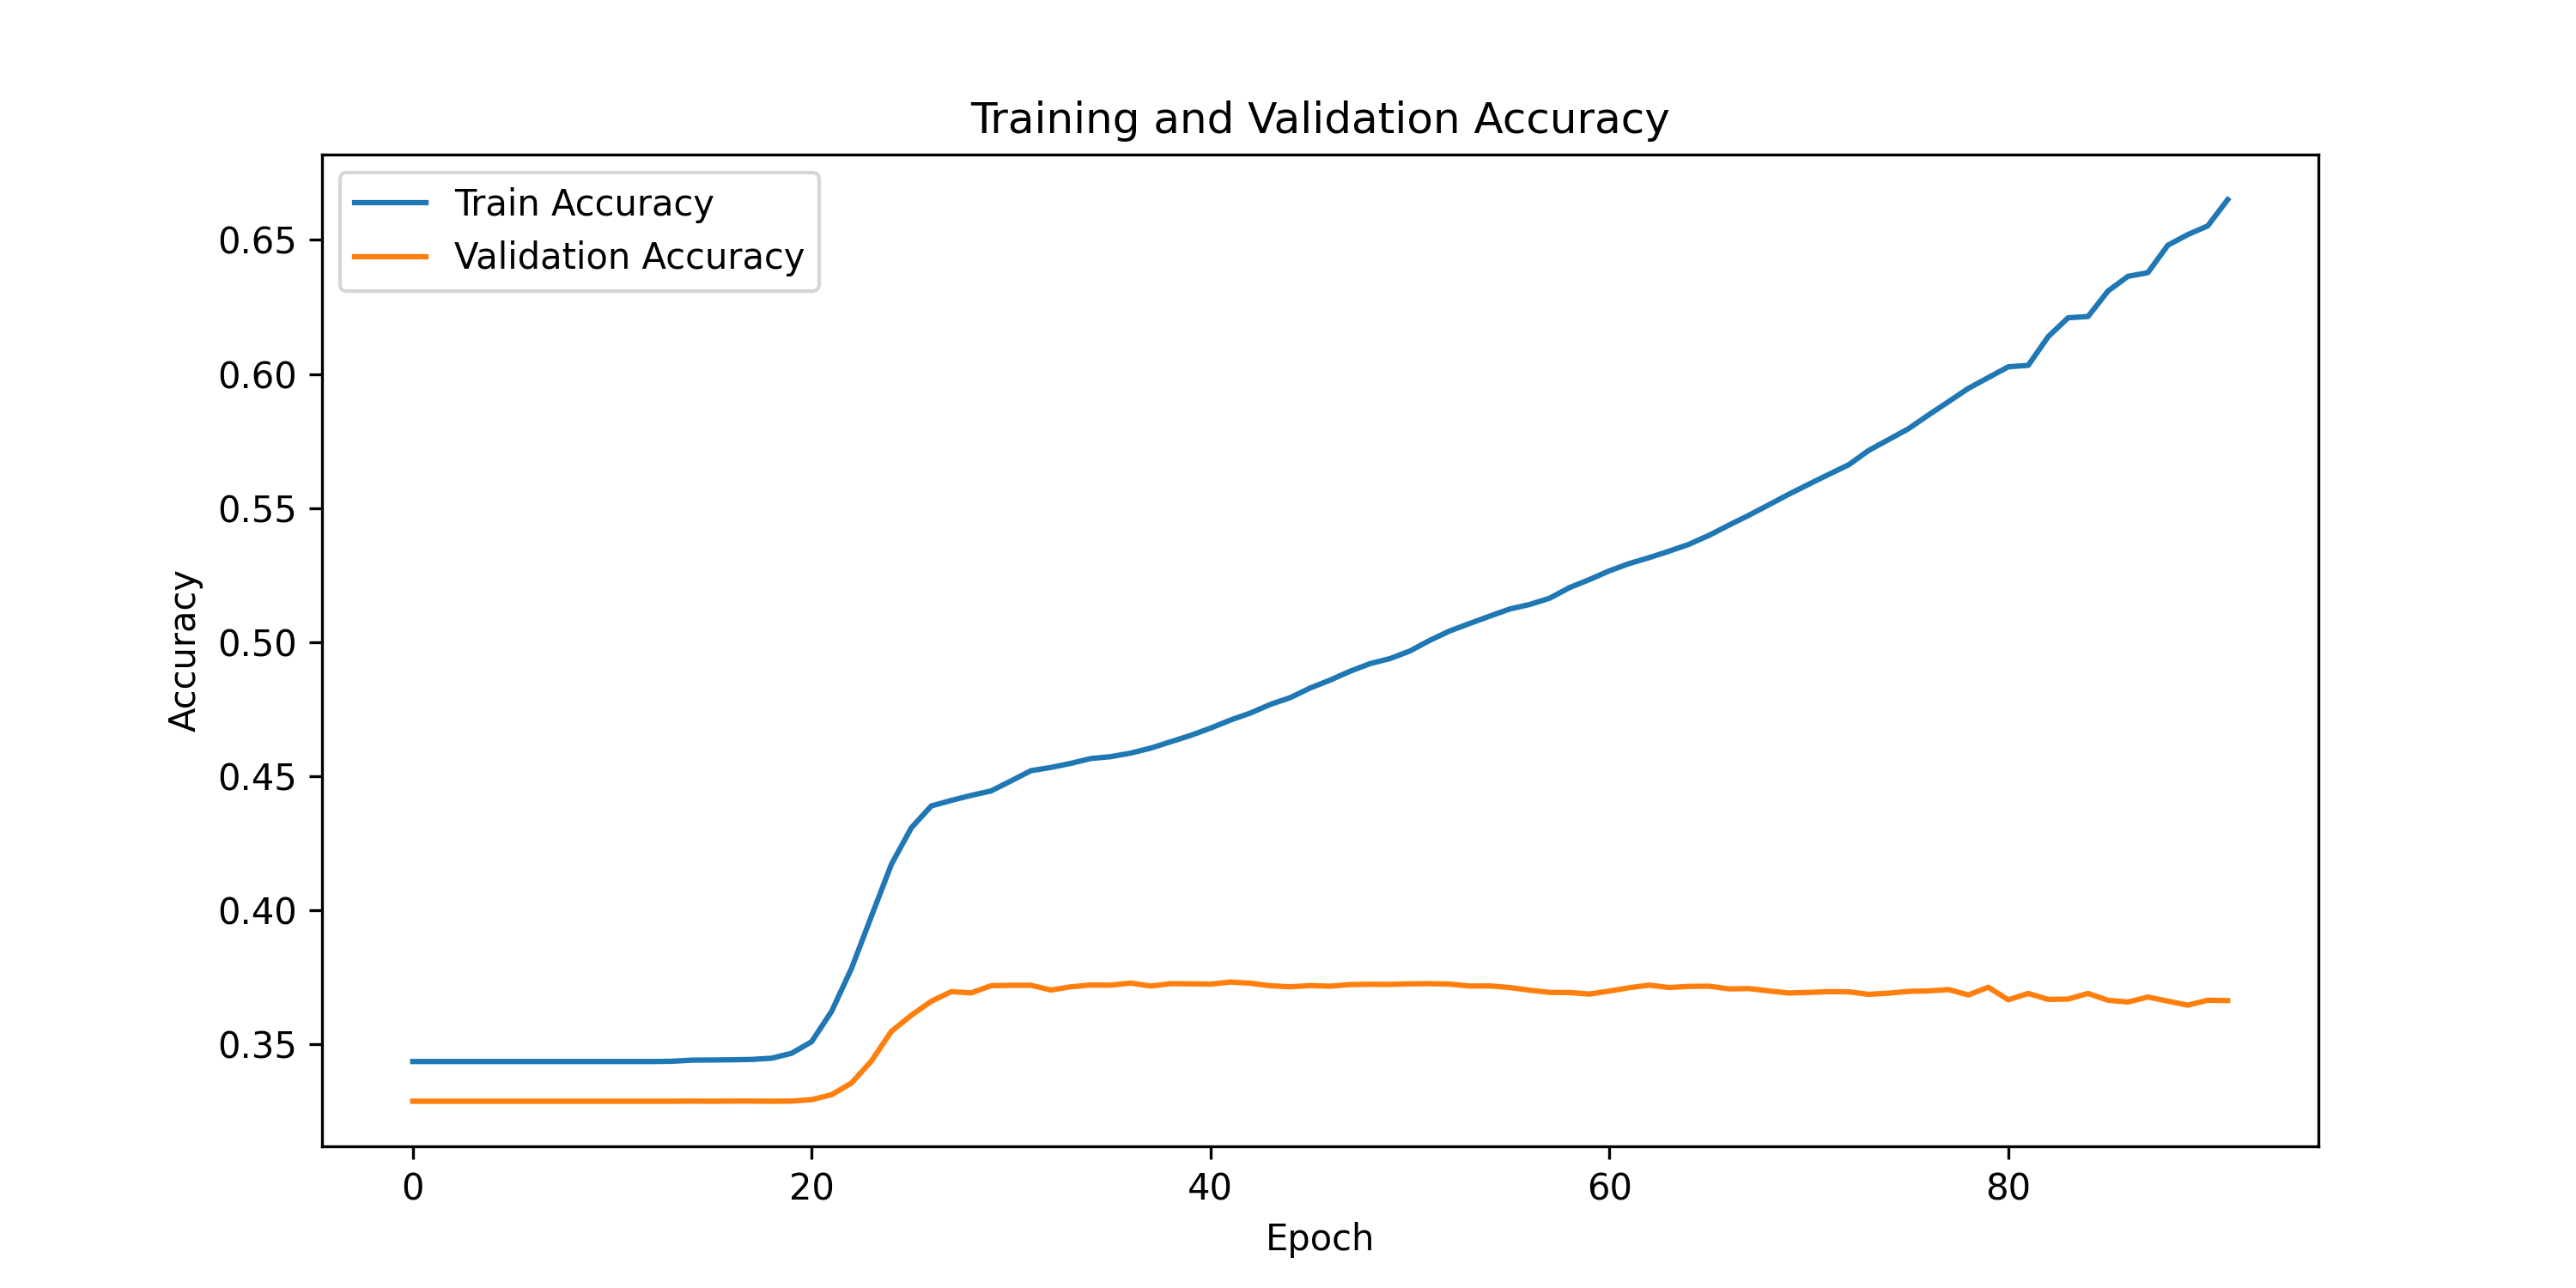
\includegraphics[width=1\textwidth]{Images/accuracy_curves_noSVD.png}
    \caption{Validation Accuracy vs Number of Epochs for MLP Model}
    \label{fig:mlp_val_acc}
\end{figure}

As shown above, there was severe overfitting with large 
numbers of epochs.
To combat this, the model parameters were saved after each epoch,
and the model with the highest validation accuracy was used for testing.
The model achieved RMSEs of 0.788 for the training data, 1.17 
for the validation data, and 1.094 for the test data. 
Results are shown in Table \ref{tab:results}.


Lastly, the algorithms were run with SVD, which reduced the 
number of features from 2668 to 991. This was chosen as it captured 95\%
of the variance in the data. A plot of the variance explained by each
SVD component is shown in Figure \ref{fig:svd_variance}.
\begin{figure}[H]
    \centering
    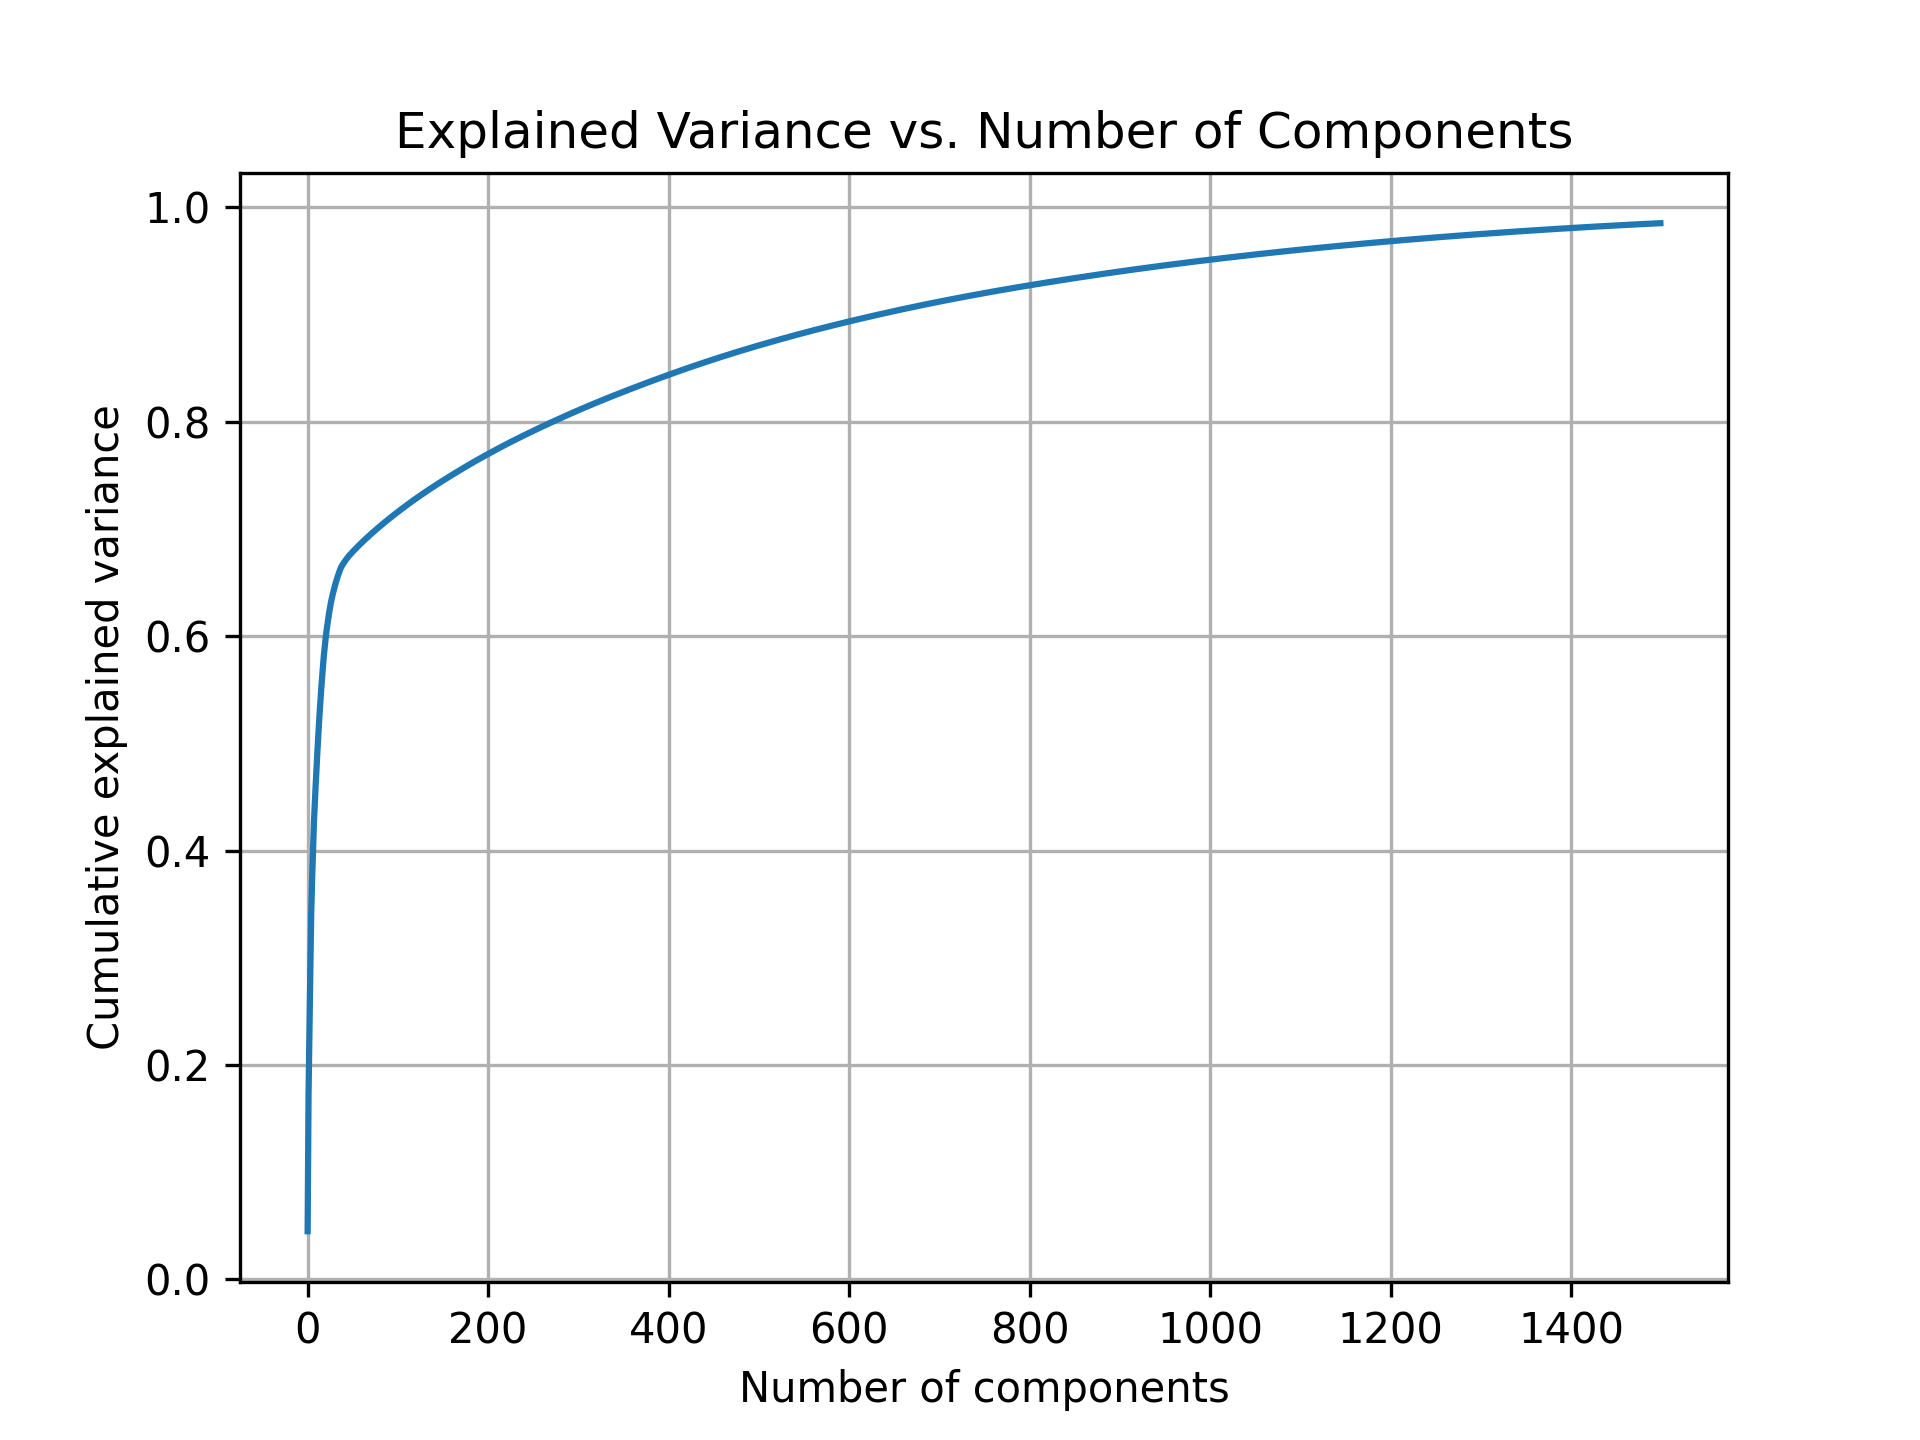
\includegraphics[width=0.8\textwidth]{Images/SVDPlot.png}
    \caption{Variance Explained by Each SVD Component}
    \label{fig:svd_variance}
\end{figure}


Both the logistic regression and MLP models
were able to achieve similar results to the models without SVD, although 
they were slightly worse. Results for all models are shown in Table \ref{tab:results}.



\begin{table}[H]
    \centering
    \caption{Results of Logistic Regression and MLP Models}
    \label{tab:results}
    \setlength{\tabcolsep}{3pt}
    \begin{tabular}{lccccccc}  % Changed from lccc to lccccccc (8 columns)
        \toprule
        Model & SVD & Train Acc & Val Acc & Test Acc & Train RMSE & Val RMSE & Test RMSE \\
        \midrule
        Logistic Regression & No & 0.487 & 0.37 & 0.415 & 1.045 & 1.139 & 1.123 \\
        MLP & No & 0.471 & 0.373 & 0.416 & 0.788 & 1.17 & 1.094 \\
        Logistic Regression & Yes & 0.456 & 0.361 & 0.399 & 1.09 & 1.151 & 1.141 \\
        MLP & Yes & 0.478 & 0.368 & 0.403 & 0.736 & 1.21 & 1.118 \\
        \bottomrule
    \end{tabular}
\end{table}
The MLP model was able to achieve the best results, with a test 
RMSE of 1.094, therefore this is the final model that is being chosen. 


\section{Discussion}
As in many machine learning tasks, data sparsity was a 
major issue contributing to the complexity of the problem.
The dataset contained a large number of users and movies, but
most users only rated a small number of movies, and most movies 
were rated by a small number of users. This resulted in a 
sparse dataset, which increased the dimensionalty of the input,
even though the inherent dimensionality of the problem was much lower. This 
can be seen in the number of features, which was 2668 before SVD
and 991 after SVD. The models were able to achieve similar results
 with and without SVD, showing that the input data after 
 passing through SVD did in fact represent the original data well. Since
 computationally complexity of many common algorithms scales poorly 
 with the number of features, the sparsity can drastically increase the 
time it takes to train a model for real world applications.


\end{document}